\addcontentsline{toc}{subsection}{Block-length}
\subsubsection*{Block-length } 

The block-length selection is crucial in a GEV analysis. It is important to choose a block-length which is large enough for the limiting arguments supporting the GEV approximation (\ref{exttheom}) to be valid, or else a large bias in the estimates could occur. Since a large block-length implies less data to work with and thus a large variance of the estimates, a compromise must be found as noted in \hyperref[sec::1]{Chapter \textbf{\ref{sec::1}}}. Here, we chose yearly blocks, justifiable for the above reason and for their interpretability and ease of use.
Note that this will cause wastage of data since we will not be using 6 months (from October to March) in the analysis since it did not have an annual maximum. 
One way to prevent this wastage could be by fitting several GEV models on some subsets of the dataset divided by a seasonal criterion, but this approach would generate other issues. 



\addcontentsline{toc}{subsection}{R packages for EVT}
\subsubsection*{R packages in EVT}

A bunch of packages exist for modeling extreme values in R. We have explored and used most of them to do the following analysis, and made some comparisons. Regarding classical EVT analysis, we must name the following : 

\begin{itemize}
	\item[$\vartriangleright$] \texttt{ismev}, \texttt{evd}, \texttt{extRemes} (good for a wide nonstationary analysis with POT and nice tutorials, see e.g. \citet{gilleland_extremes_2016}), \texttt{POT} (see \citet{ribatet_users_2006}), \texttt{evir}, \texttt{fExtremes}, $\dots$
\end{itemize}
Since a number of packages are doing the same analysis but with different methods, we decided to rely mostly on \texttt{ismev} as it is the package used in the book of \citet{coles_introduction_2001}.

\section{Inference of the Stationary Model}\label{sec:xpstatio}

\hyperref[sec::1]{Chapter \textbf{\ref{sec::1}}} is important to understand the concepts used in this section but we will now be mostly based on inferential methods discussed in \hyperref[sec::gevinfernce]{Section\textbf{ \ref{sec::gevinfernce}}}, return levels in \hyperref[rlgev]{Section\textbf{ \ref{rlgev}}} and diagnostics in \hyperref[sec:diag]{Section\textbf{ \ref{sec:diag}}}.

\subsection*{Maximum Likelihood}\label{sec:mlepratic}

We estimate the MLE's relying on packages cited above, but also by checking it manually, that is by numerically solving the minimization of the negative log-likelihood. This can be done with the \texttt{nlm} routine using the Newton-Raphson algorithm of \citet{dennis_numerical_1987}. This algorithm is based on an approximation of the log-likelihood by a quadratic function which is the second order Taylor series approximation of the log-likelihood for a given point.
Estimates and standard errors are shown in Table \ref{tab:estlik}.

\begin{table}[!htbp] \centering 
	\caption{MLE's of the three GEV parameters assuming a independent (stationary) context.} 
		\vspace{-.1cm}
	\label{tab:estlik} 
	\begin{tabular}{@{\extracolsep{5pt}} cccc} 
\toprule 
		& Location $\mu$ & Scale $\sigma$ & Shape $\xi$ \\ 
\midrule
		Estimates (s.e.) & $30.587$ ($0.216$)& $2.081$ ($0.155$) & $\boldsymbol{-0.254}$ ($0.067$) \\ 
\bottomrule
	\end{tabular} 
\end{table} 
\vspace{-.1cm}
Table \ref{tab:estlik} the negative value of the \textbf{shape} parameter, meaning that we are under a Weibull-type of the GEV family. From Figure \ref{gevdens} the corresponding density has the form of the red line which has a finite right endpoint.
A likelihood ratio test will confirm this in Table \ref{tab:comp_mod0}, comparing the fitted EV-Weibull with a Gumbel distribution.

The Weibull-type implies that the fitted distribution has an estimated right endpoint of $\hat{x}_*=\hat{\mu}-\hat{\sigma}\cdot\hat{\xi}^{-1}=38.77^{\circ}c$. Comparing this value with the maximum value of the annual series ($36.6^{\circ}c$) shows that this model takes into account the uncertainty since there are only $116$ years of data. Hence, it allows return levels, i.e. quantiles of the fitted distribution, to go beyond $36.6^{\circ}c$, for very long return periods. This will be highlighted in Figure \ref{fig:rl_empdes} (right plot) where we notice a probability mass beyond the minimum and the maximum values of the series from the fitted model.


\paragraph*{Profile log-likelihood intervals} 
These intervals are often preferred for individual parameters to handle the poor normal approximation of the MLE. Results provided by the \texttt{ismev} package are in Figure \ref{fig:proflikpar} left in \hyperref[app:fig]{Appendix \textbf{\ref{app:fig}}}.
These intervals are constructed by searching for the horizontal line and then subtracting the maximum log-likelihood by half the corresponding upper quantile of the $\chi^2_{\text{df}}$ for $\text{df}=1$ parameter of interest. We notice that :
\begin{itemize}
	\item Even at $99\%$ confidence, the interval for $\hat{\xi}$ does not contain $0$ supporting that the distribution is left heavy-tailed and right bounded.
	
	\item $95\%$ intervals for the location and scale parameters are $[30,\ 31]$ and $[1.8, \ 2.4]$ respectively.
	
	\item The intervals do not present many asymetries. In fact, these will be more relevant for return levels as we will see in the \hyperref[sec:rlemp]{next Section}.
\end{itemize}


\subsection*{Probability-Weighted-Moments}

It is always good practice to check whether different methods lead to significantly different results.
A second estimator we have seen is the \emph{probability-weighted-moments}. Results are shown in Table \ref{tab:estpwm}.


\begin{table}[!htbp] \centering 
	\caption{Stationary GEV parameters estimated by PWM.} 
		\vspace{-.1cm}
	\label{tab:estpwm} 
	\begin{tabular}{@{\extracolsep{5pt}} cccc} 
\toprule
		& Location $\mu$ & Scale $\sigma$ & Shape $\xi$ \\ 
\midrule
		Estimates & $30.552$ & $2.115$ & $\boldsymbol{-0.232}$ \\ 
\bottomrule
	\end{tabular} 
\end{table} 
\vspace{-.1cm}
We immediately see that these results are very close to the MLE's of Table \ref{tab:estlik}, in particular for the EVI $\xi$. This gives us confidence that we are indeed under a Weibull-type GEV model. For convenience and for their properties, we will only keep the MLE's to work with in the following.



\subsection{Return Levels}\label{sec:rlemp}

First presented in \hyperref[rlgev]{Section \textbf{\ref{rlgev}}}, return levels are appreciated by the practitioners for inference in an environmental EVT context.
Usual likelihood intervals relying on the normal approximation are not reliable for return levels. Hence, we decided to compute the profile likelihood intervals and compare both values in Table \ref{tab:rl1}.


\begin{table}[!htbp] \centering 
	\caption{The $m$-year return level estimates and $95\%$ intervals. Last line computes the length's differences between the normal and the profile likelihood intervals.} 
	\vspace{-.1cm}
	\label{tab:rl1} 
	\begin{tabular}{@{\extracolsep{5pt}} ccccc} 
\toprule

		&  $2$-year & $10$-year & $100$-year & $1000$-year  \\
\midrule
		\textbf{Estimates}&$ 31.315$ & $34.153$ & $36.229$ & $37.982$ \\
		 Normal interval & $(30.88, 31.75)$ & $(33.63, 34.67)$ & $(35.21, 37.25)$ & $(35.67, 39.04)$\\ 
	    Profile likelihood interval & $(31.16, 31.68)$ & $(33.95, 34.74)$ & $(35.54, 37.84)$ & $(36.58, 40.25)$  \\
		\textbf{Difference of lengths} & $0.348$ & $0.247$& $-0.260$ & $-0.294$ \\ 
\bottomrule
	\end{tabular} 
\end{table} 

Table \ref{tab:rl1} demonstrates that, for example, the estimated $100$-year return level is $36.23^{\circ} c$ which is the temperature that will be exceeded on average once every $100$ years. However, note that very long term extrapolation should be tempered by caution since we only have $116$ years of data and predicting far beyond this value is unreliable. We can see the shift of the profile likelihood confidence intervals compared with the
normal intervals. This can also be seen on the return level plot in Figure \ref{fig:rl_empdes} where we see blue dots going higher than red lines for higher return periods. We also see that the profile likelihood intervals are more precise %\footnote{In the sense of a narrower confidence interval. A Monte-Carlo study of accuracy could be made using observed data.}
 for small return periods, i.e. approximately below half the total number of annual data, and then profile likelihood intervals become wider than normal intervals. This illustrates how profile likelihood intervals better take into account the uncertainty of long-term predictions.
Hence, in addition to arguments already provided, uncertainty but also climate warming lead us to have a preference for profile likelihood intervals which, surprisingly, are not used by default in EV packages such as \texttt{ismev}.


\subsection{Diagnostics}

\hyperref[sec:diag]{Section \textbf{\ref{sec:diag}}} provided the tools to check the accuracy of the fitted model. The goal here is to check that the
model $\hat{F}$ fitted by MLE is accurate enough for the true distribution $F$ which is estimated by the empirical df
(\ref{eq:emprdist}). First, we present the quantile and the probability plots in Figure \ref{fig:ppqqplot}.

\begin{figure}[!htb]
	\centering	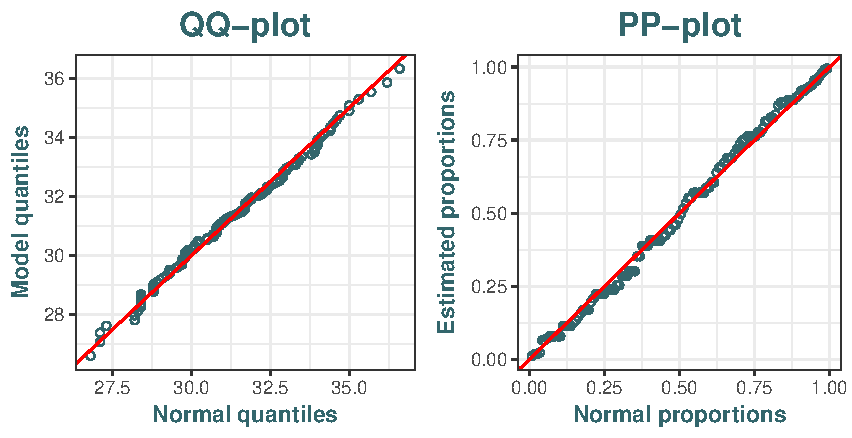
\includegraphics[width=.7\linewidth]{pp_qqplot.pdf}\caption{Quantile (left) and probability (right) plots for the stationary GEV model fitted by MLE.}\label{fig:ppqqplot}
\end{figure}

Both plots show points lying very close to the unit diagonal, showing that the empirical df is very close to the fitted model and hence putting confidence that our model fits our data accurately.
The right plot in Figure \ref{fig:rl_empdes} has a similar interpretation and leads to the same conclusion, although the fitted model has a higher peak.

\begin{figure}[!htb]
	\centering	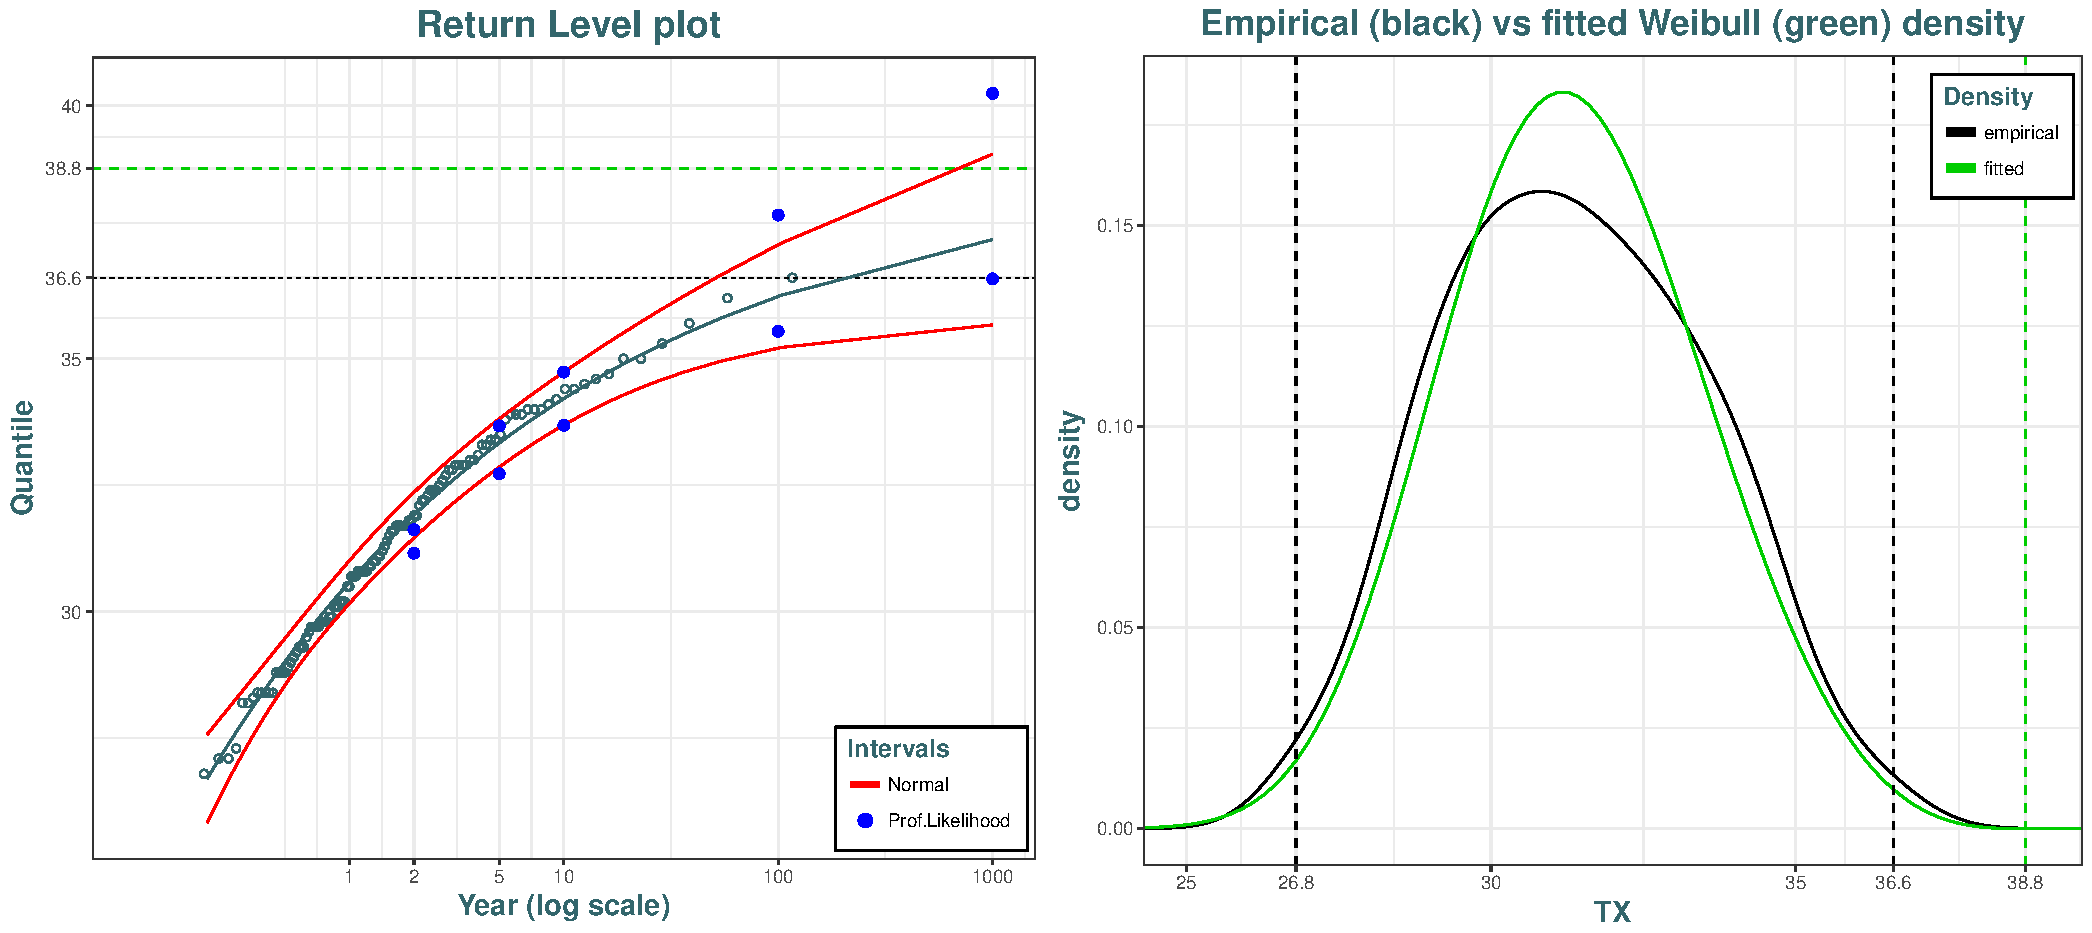
\includegraphics[width=.75\linewidth]{rl_empdes.pdf}\caption{(Left) Return level plot with red lines representing normal confidence intervals, and blue points the individual profile likelihood intervals for return levels. The horizontal dotted line represents the right endpoint of the	fitted model in green and the maximum of the series in black. (Right) kernel density in black compared with the density of the fitted model in green, with dotted lines representing the \textbf{endpoints} of the empirical distribution, and green doted lines still represent the same right endpoint of the fitted EV-Weibull. A Gaussian kernel with a bandwidth calculated by the \citet[pp.48, (3.31)]{silverman_1986} "rule of thumb" has been used.}\label{fig:rl_empdes}
\end{figure}


\subsection*{Return Level Plot}

Another tool that is available in EVT to check the fit of a model is the return level plot. It allows for comparisons of
observations with return levels coming from the EV-Weibull model fitted by MLE. The left plot in
Figure \ref{fig:rl_empdes} shows us a concave shape of the return levels with the return period wich asymptotes to the right endpoint $x_*$ of the model since $\xi<0$. Note that all points are very close to the estimated return level and hence we have confidence that our model
is suitable. Moreover, all these points are inside the normal confidence intervals (recall that profiled intervals are not suitable for very small return periods).

Whereas the estimated return level cannot go beyond $x_*$, we see that for very high return periods, the upper bound of the confidence intervals goes beyond this right endpoint of the fitted model. Again, this is justified since for such far periods, both intervals are allowed to go beyond the domain of the fitted model, with profile likelihood ones taking more uncertainty into account.



\subsection*{Profile Likelihood Intervals for Return Levels}

Figure \ref{fig:proflikrl} left in  \hyperref[app:fig]{Appendix \textbf{\ref{app:fig}}} represents the profile log-likelihood intervals for three return periods, at the $x$-intersections between the blue line and the curve. We
can see the asymmetries (positive skew) which are increasing at higher
values of the return period. This was expected since the data at hand provides increasingly weaker information about high return levels of the process. We also displayed the return levels
from Table \ref{tab:rl1}  represented by green lines on the plots in Figure \ref{fig:proflikrl}, and which were computed relying on another method from the
package \texttt{extRemes}. It is interesting to see how the results can be slightly different.


\subsection{Stationary Analysis}

\hyperref[sec:statio]{Section \textbf{\ref{sec:statio}}} proved that a dependent sequence can still have the GEV distribution in the limit of normalized maxima. This will only induce different location and scale
parameters compared to the sequence as if it were independent.
We can visualize dependence in the series for example with the autocorrelation functions. Corresponding plots are shown in Figure \ref{fig:acf_gev} let in \hyperref[app:fig]{Appendix \textbf{\ref{app:fig}}} where we see that temporal dependence is light, but present. 
Actually, estimates shown in Table \ref{tab:estlik} implicitly take this dependence into account. 

\addcontentsline{toc}{subsubsection}{POT}
\subsubsection*{POT}

 Dependence is not a big concern for GEV, however it is more problematic for POT. Indeed, by only analyzing data that are above a threshold (say $30^{\circ}c$), serial dependence in the data can be strong and observations will have the tendency to occur in clusters. We illustrated this in Figure \ref{fig:abo} in \hyperref[app:fig]{Appendix \textbf{\ref{app:fig}}} which highlights this dependence with red lines corresponding to the historic heat waves of summers 1911 and 1976 in Uccle. Indeed, observations lying on the red lines are serially correlated since they occurred during a same period of extreme heat. It is not difficult to assume that \emph{hot days are more likely to be followed by hot days}.
 
Moreover, we estimated the extremal index $\theta$ by the method of \citet{ferro_inference_2003} to get an idea of the extent of this extremal dependence. We obtained $\hat{\theta}\approx 0.42$ and hence, one interpretation is that the extremes are expected to cluster by groups of mean size $0.42^{-1}\approx 2.4$. We can visualize from Figure \ref{fig:abo} that the points have indeed some tendency to form groups of size around $2$. The next step (not displayed here) is to decluster the series.



\section{Parametric Nonstationary Analysis}\label{sec:xpnp}


As depicted in the introductory Figure \ref{first_fig}, even the assumption of stationarity is likely to be poor for our data. 
Whereas the oscillatory behavior caught by the LOESS model is probably due to noise rather than a true characteristic of the underlying process, the increasing trend is more alarming. Indeed, our flexible modeling of the trend in \hyperref[sec:splines]{Section \textbf{\ref{sec:splines}}} confirmed that the trend is statistically significant for two periods when doing pointwise comparisons but it is inadequate since we proved that this method leads to coverages that did not match with the assumed confidence level. When controlling for simultaneous tests, significance of the trend completely disappeared. However, one could argue that these intervals are very large (looking back at Figures \ref{fig:post_draws} or \ref{fig:derivsplines}) and thus not precise. Hence, results are not clear regarding this trend and a nonstationary GEV analysis is worth undertaking. 




\subsection{Comparing Different Models}\label{sec:comp0}


Our first approach will use the deviance statistic by sequentially comparing nested models. The number of degrees of freedom (df) represent the number of parameters in the model (i.e., its complexity). The parametric models we will first compare are :

\begin{enumerate}
	\item \emph{Gumbel} : most simple  EV-model with unrestricted domain and only 2 parameters as $\xi=0$.
	\item \emph{stationary} : EV-Weibull model fitted in Table \ref{tab:estlik} by MLE.
	\item\label{i:linear} \emph{linear in $\mu(t)$} : allowing a nonstationary location parameter with $\mu(t)=\beta_0+\beta_1\cdot t$.
	\item \emph{quadratic in $\mu(t)$} : allowing a nonstationary location parameter with $\mu(t)=\beta_0+\beta_1\cdot t+\beta_2\cdot t^2$.
	\item \emph{linear in $\mu(t)$ and $\sigma(t)$} : same as Model \ref{i:linear} regarding the location but with nonstationary scale $\sigma(t)=\exp(\alpha_0+\alpha_1\cdot t)$. The use of the inverse link $b(\cdot)=\exp(\cdot)$ is to ensure positivity of $\sigma$ $\forall t$.
	\item \emph{cubic in $\mu(t)$} : nonstationary location parameter with $\mu(t)=\beta_0+\beta_1\cdot t+\beta_2\cdot t^2+\beta_3\cdot t^3$. Note that computational singularities occurred for the likelihood computation of this model (or more complex ones). This came from a problem of solving the hessian to compute the covariance matrix of the parameters since there were too much linear dependencies in the hessian. We solved this by decreasing the tolerance, but this shows us that a linear model with so many polynomial terms is not recommended.
\end{enumerate}
\hyperref[nstatio]{Section \textbf{\ref{nstatio}}} explains that it is not recommended to model $\xi$ as a smooth function of time, since the data provides little information about the shape of the distribution relative to the location and the scale.
The p-values from the sequential pairwise comparisons have been computed with respect to the best retained model. Results are shown in Table \ref{tab:comp_mod0}.

\begin{table}[!htbp] 
	\centering \caption{ Comparisons of nested GEV models with nonstationary parameters. Significant p-values at level $5\%$ are shown in bold.% Nonstationary linear (in the parameters) model in $\sigma(t)$ use the exponential link.
		} 
	\vspace{-.1cm}
	\label{tab:comp_mod0} 
\begin{tabular}{@{\extracolsep{5pt}} ccccc} 
\toprule
		\textbf{Model} & $\ell$ & df & p-value \\
\midrule
		Gumbel & $-256.84$  & $2$ & \\
		stationary  & $-251.75$ & $3$  & \boldsymbol{$0.14\%$} \\
		\textbf{linear in} \boldsymbol{$\mu(t)$} & $\boldsymbol{-241.81}$ & $\boldsymbol{4} $& \boldsymbol{$0.001\%$}  \\
		quadratic in $\mu(t)$ & $-241.48$ & $5$ & $42\%$ \\
		linear in $\mu(t)$ and $\sigma(t)$ & $-241.69$ & $5$ & $63\%$ \\
		cubic in $\mu(t)$ & $-241.37$ & $6$ & $65\%$ \\
\bottomrule
\end{tabular}
 	\vspace{-.15cm}
 \end{table} 
The model that is chosen by this procedure in Table \ref{tab:comp_mod0} is Model \ref{i:linear} which allows a linear model for the location parameter. The choice is clearly emphasized by likelihood ratio tests and hence we have confidence in a nonstationary GEV model with a linearly increasing trend from the location. In the \hyperref[sec:nnxp]{next Section} we will allow for more flexibility in the model's parameters.
\iffalse
\begin{itemize}
	\item Variation in time through t accounting for the season : $\mu (t)=\beta_0+\mathbbm{1}_i(t)$ where i=1,2,3,4 represent each seasons.
\end{itemize}
This is more appropriate in threshold exceedance models.
\fi



\subsection{Selected Model : Diagnostics and Inference} 

Having selected the best model, we will now give estimates of the new parameters before assessing the accuracy of this new model in order to provide reliable inferences through return levels.


\subsubsection*{Model}

Table \ref{tab:estliknsta} shows the parameters and standard errors for the selected nonstationary GEV model estimated by MLE. 

\vspace{-.05cm}
\begin{table}[!htbp] \centering 
	\caption{MLE's of the nonstationary GEV parameters of Model \ref{i:linear} with a linear trend on $\mu(t)=\beta_0+\beta_1\cdot t$.} 
	\vspace{-.2cm}
	\label{tab:estliknsta} 
	\begin{tabular}{@{\extracolsep{5pt}} ccccc} 
\toprule
		& Location $\beta_0$ & Location $\beta_1$ & Scale $\sigma$ & Shape $\xi$ \\ 
\midrule
		Estimates (s.e.) & $29.13$ ($0.38$)& $0.0254$ ($0.005$) & $1.87 (0.14)$ & $-0.21$ ($0.06$) \\ 
\bottomrule
	\end{tabular} 
\end{table} 

We notice that $\xi$ is in the same range as previous stationary model. The parameter $\beta_1$ says that the location parameter $\mu(t)$ is expected to increase by $0.025$ each year, starting at $\beta_0=29.13$ until $29.13+0.025\cdot 116=32.07$ where $116$ is the number of years of data. Extrapolation, say in year $2050$ for example, would then lead to a distribution GEV($32.93,1.87,-0.21$), other parameters being held constant.


\subsubsection*{Diagnostics}

\hyperref[sec:gev_nonstatio]{Section \textbf{\ref{sec:gev_nonstatio}}} showed how diagnostic tools such as quantile and probability plots can still be used in a nonstationary context, with some transformations, i.e. the observations must be standardized to have a Gumbel distribution.
Results are shown in Figure \ref{fig:ppqqplot2} for the selected model.

\begin{figure}[!htb]
	\centering	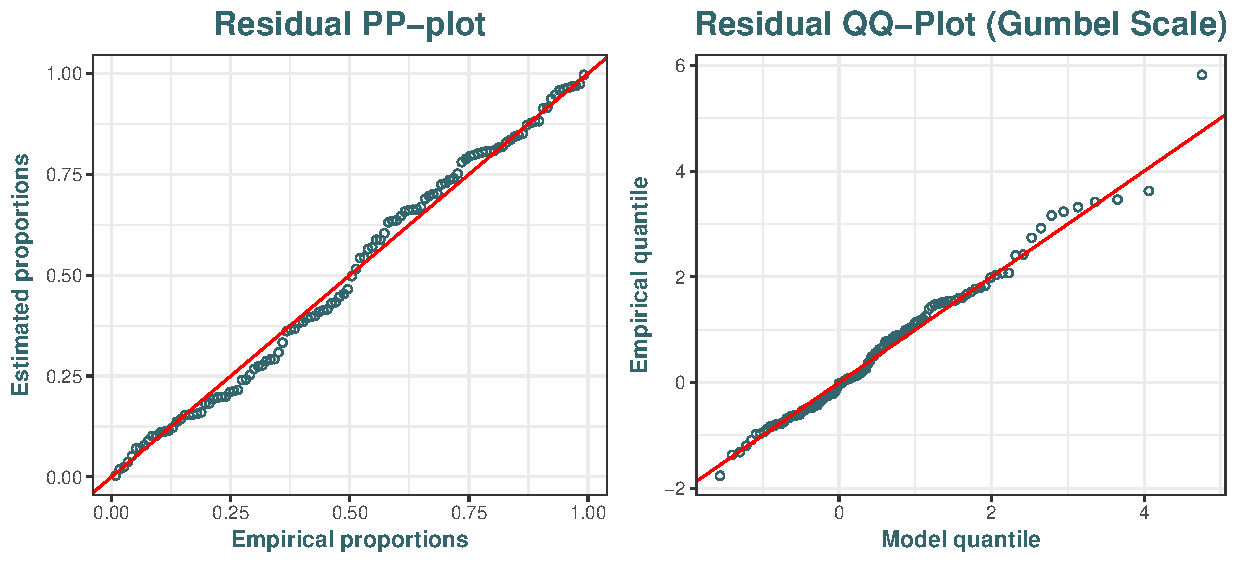
\includegraphics[width=.7\linewidth]{ppqq_trans.pdf}\caption{(left) Residual probability plot and (right) residual quantile plot on the Gumbel scale for the nonstationary GEV model allowing for a linear trend in the location parameter fitted by MLE.}\label{fig:ppqqplot2}
\end{figure}


We appreciate that the fit seems accurate. Note that problems for large quantiles in the residual QQ-plot is not problematic. 


\subsubsection*{Return Levels}



\begin{wrapfigure}[12]{r}{0.45\textwidth}
	\centering
	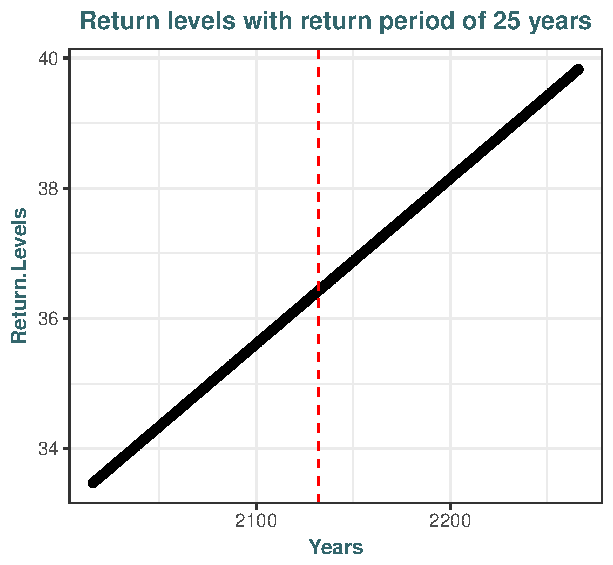
\includegraphics[width=0.42\textwidth]{rl_nsta.pdf} % 6.64x5.17 inches
	\caption{Return levels (in blue) of the nonstationary GEV model allowing linear trend on $\mu(t)$. Dotted red line represent horizon after $n=116$ years and black lines represent the series $[1980-2016]$.  }
	\label{fig:rl_nsta}
\end{wrapfigure}

We will still use the return levels as our reference tool to make inference in EVT, even in the presence of nonstationarity. Since the distribution will change every year (by a right shift of the location), the return levels will also change each year. Hence, we plot return levels against years by choosing a $10$-year return period which corresponds to the $90\%$ quantile of the fitted GEV distribution. This is shown in Figure \ref{fig:rl_nsta}.

We clearly see the linear pattern of the return levels with $t$ explained by the linear model for $\mu(t)$. The $x$-axis has been carefully chosen to have the best interpretation. $36$ years are in the range of data and then return levels are extrapolated from the model. The maximum prediction horizon of length $183$ corresponds to the reach of $40^{\circ}c$ for the $10$-year return level. 

Quite interestingly, we see that the fitted return level after $n=116$ years, where $n$ is the number of data, is $38.3^{\circ}c$, which is higher than the maximum $36.6^{\circ}c$ of the series. 
This return level means that, in year $2132$, we will expect a maximum temperature of $38.3^{\circ}c$ to be reached in a period of $10$ years. Note that such far extrapolation, especially those right to the number of data (dotted red line), should be made with caution.
Moreover, we cannot know in practice whether or not it is believable
for the upward linear trend in annual maximum temperatures to continue to be valid beyond the range of data.

\section{Improvements with Neural Networks}\label{sec:nnxp}


New advances in EVT enables consideration of more flexible approaches. Indeed, we have seen that a linear model in the location parameter is significant against the other parametric models of Table \ref{tab:comp_mod0}, but we did not consider enough models to be able to sustain this conclusion.

As discussed in \hyperref[sec:gevcdn]{Section\textbf{ \ref{sec:gevcdn}}}, Neural Networks (NN) allow through a complex process to capture complex relationships between the input (time) and the outputs (the 3 GEV parameters). We will follow the approach of \citet{cannon_flexible_2010} and its package \texttt{GEVcdn} using an extension of the multi layer perceptron, the GEV Conditional Density Network (GEV-CDN).

Model parameters are estimated from weights and biases via GML using a quasi-Newton BFGS optimization algorithm and appropriate relationships, i.e. refer to Figure \ref{NN} for the complete architecture. 
To avoid convergence to a shallow local minimum of the error surface, the algorithm is run $100$ times with different initial values.
The selected model is the one that minimizes an appropriate cost-complexity criteria ($\text{AIC}_{\text{c}}$ or BIC). Different structures are tested with combinational cases of stationary and nonstationary parameters of the GEV distribution, or linear and nonlinear architecture of the CDN. 


\subsection{Models and Results}


NN's are meant to approximate any functions with very good accuracy. Thus, it incorporates all the parametric models considered so far. We allowed the shape parameter $\xi$ to vary with time in order to consider all possible models, though this is not advised for EV models as it allows the family of the fitted distribution to change with time. In any case, it does not change the final result. 

Figure \ref{NN} represented the fully connected architecture. The hierarchy of models we will consider is, by ascending complexity :

\begin{enumerate}
	\item\label{mod111} Stationary GEV model as in Table \ref{tab:estlik}, but now fitted by \textbf{G}ML.
	
	\item\label{mod222} Nonstationary GEV  model with linear trend on the location. 
	\item Nonstationary GEV model with linear trend on the location and the scale parameters.
	
	\item\label{mod444} Nonstationary GEV model allowing complete linear relationships for the location, scale and shape parameters.
	
	\item[5.-9.]\label{i:nonlin} The preceding nonstationary models allowed linear relationships between time and the parameters since the activation function $m(\cdot)$ used to compute the hidden layer nodes (\ref{eq:nnlay1}) was the identity link. Now, since $m(\cdot)$ is a (logistic) sigmoid function, the relationships can be nonlinear. The degree of complexity of the nonlinear relationships, i.e. number of degrees of freedom of the model, is controlled by the number of hidden layers. We also implemented the hyperbolic tangent as activation function but it has not improved the results.
\end{enumerate}
Models \ref{mod222} to \ref{mod444} thus allow \textbf{linear} relationships of the parameters with time while the following Models \hyperref[i:nonlin]{5 to 9} can handle nonlinear relationships.
We did not consider nonstationary models for the sole $\sigma(t)$ parameter as it would not correspond to the goal of this thesis, in the sense that allowing changes in scale but not in location would be irrelevant. 

We picked the recommended values of $6$ and $9$ for the parameters $c_1$ and $c_2$ (resp.) of the Beta prior (\ref{eq:betaprior}) for $\xi$ to compute the generalized likelihood (\ref{eq:gml}). Moreover, 
\citet{cannon_flexible_2010} recommended to use between 1 and maximum 3 hidden layers due to the relatively small sample size $n=116$ and the danger to quickly overfit. Table \ref{tab:comp_mod} displays the results for maximum 2 hidden layers.


\begin{table}[!htbp] 
	\centering \caption{Comparisons of nonstationary GEV-CDN models fitted by GML. Linear models have the identity activation function and the nonlinear models have the logistic sigmoid activation function. } 
	\label{tab:comp_mod} 
	\hspace{-2.5cm}
\begin{tabular}{@{\extracolsep{5pt}} rccccc} 
	\cmidrule[\heavyrulewidth]{2-6}
 &	\textbf{model} & $\text{AIC}_{\text{c}}$ & BIC & hidden & df \\
	\cmidrule{2-6}
	
	& stationary & -19.6 & -11.5 & 0 & 3 \\ 
	\multirow{3}{*}{Linear $\begin{dcases*} \\ \\  \end{dcases*}$} 
	&$\mu(t)$ & -$37.4$ & -$\boldsymbol{26.7}$ & $0$ & $4$  \\ \hspace{-0.5cm}
	&$\mu(t)$, $\sigma(t)$ & -35.4 & -22.2 & 0 & 5 \\
	&$\mu(t)$, $\sigma(t)$, $\xi(t)$ & -34.2 & -18.4 & 0 & 6 \\
	
	 \multirow{6}{*}{\textcolor{LimeGreen}{Nonlinear} $\begin{dcases*} \\ \\ \\ \\ \\ \end{dcases*}$} &	$\mu(t)$ & -35.4 & -19.6 & \textcolor{LimeGreen}{1} & 6 \\
	&$\mu(t)$, $\sigma(t)$ &  -36.2  & -17.9 & \textcolor{LimeGreen}{1} & 7 \\ 
	&$\mu(t)$, $\sigma(t)$, $\xi(t)$ & -34 & -13.3 & \textcolor{LimeGreen}{1} & 8 \\
	&$\mu(t)$ & -37.4 & -14.3 & \textcolor{LimeGreen}{2} & 9 \\
	&$\mu(t)$, $\sigma(t)$ & -32.5 & -4.7 & \textcolor{LimeGreen}{2} & 11 \\
	&$\mu(t)$, $\sigma(t)$, $\xi(t)$ & \textbf{-38.4} & 3.9 & \textcolor{LimeGreen}{2} & 13 \\		\cmidrule[\heavyrulewidth]{2-6}
\end{tabular}
\end{table}

Relying on the BIC, Table \ref{tab:comp_mod} reinforces the findings of Table \ref{tab:comp_mod0}. This criterion is justified because the $\text{AIC}_{\text{c}}$ does not penalize sufficiently complex models and we want a parsimonious model since NN models are likely to overfit. Indeed, the $\text{AIC}_{\text{c}}$ selected the most complex model with 2 hidden layers and 13 df, and the likelihood ratio tests always chose Model \ref{mod222} ; p-value = $10^{-4}$ when compared with the complex model chose by $\text{AIC}_{\text{c}}$.
 	
For Model \ref{mod222} selected by BIC, Table \ref{tab:estnn} shows the parameters estimated by GML from the estimation of the weights $\boldsymbol{w}^{(1)}$ and $\boldsymbol{w}^{(2)}$ with (\ref{eq:nnlay1})-(\ref{eq:nnlay2}). 

\begin{table}[!htbp]
	 \centering 
	\caption{Estimation by GML of the nonstationary parameters from the GEV-CDN Model \ref{mod222} allowing a linear trend on the location $\mu(t)=\beta_0+\beta_1\cdot t$.} 
	\label{tab:estnn} 
	\begin{tabular}{@{\extracolsep{5pt}} ccccc} 
		\toprule
		& Location $\beta_0$ & Location $\beta_1$ & Scale $\sigma$ & Shape $\xi$ \\ 
		\midrule
		Estimates& $29.11$& $0.0253$ & $1.84$ & $-0.185$ \\ 
		\bottomrule
	\end{tabular} 
\end{table} 
We notice that Table \ref{tab:estliknsta} leads to very similar results. Small differences are due to the method of estimation since we used GML here while the parametric nonstationary analysis in Table \ref{tab:estliknsta} used ML. Scale and shape parameters are of the same order of magnitude, and the same conclusions can be drawn since we used the identity activation function with no hidden layers. 
 %(mis aussi ds chap3) "Another pitfall is its lack of interpretation of the relationships retrieved by the model between inputs and outputs but it bears noting that sensitivity analysis methods as in \citet{cannon_graph_2002} could be used to identify the form of nonlinear relationships between covariates and GEV distribution parameters or quantiles."
This model does not use all the power of NN's, being more convenient to use. Nonlinear relationships retrieved from hidden layers are indeed difficult to interpret. Some quantiles of the model are shown on the left plot of the following Figure \ref{fig:bag}.
 
 
 
 \subsection{Bagging}\label{sec:xpbagg}
 
 A solution presented in \hyperref[sec:bagg]{Section \textbf{\ref{sec:bagg}}} to prevent overfitting is \emph{bagging}.
Since the linear model is not complex enough to require bagging, and the support for the linear model was not straightforward
 when looking at the  $\text{AIC}_{\text{c}}$, we will now allow for nonlinearities that will be handled by the bagging process in order to limit overfitting. From Table \ref{tab:comp_mod}, we chose 2 hidden layers to keep the model relatively simple, and we only allowed the location and scale parameters to vary with time for the reasons above. 
 
 We made use of parallel computing through the \texttt{foreach} and \texttt{doParallel} framework. This method is computationally intensive and it is important to have a reliable number $M$ of boostrap resamples for the method to be effective. It decreased computation time by a factor of $\approx 2.5$ and allowed us to have $M=1000$ resamples in only $\approx 158$ seconds\footnote{All computations are made on a \texttt{i7-7700HQ 2.8GHz 20gb ddr4}.}.
 
 We tried to estimate the parameters in Table \ref{tab:estnnbag} in \hyperref[app:fig]{Appendix \textbf{\ref{app:fig}}}.
 But, from the nonlinear relationships introduced in the model, it was not possible to accurately estimate the parameters $\mu(t)$ and $\sigma(t)$. Sensitivity analysis methods such as proposed by \citet{cannon_graph_2002} are recommended to yield more accurate estimates of the parameters.
 We note that, the scale parameter is (slightly but) constantly decreasing with time, whilst we expected that the climate warming would lead to more variable extremes.
 
 Results of the generated quantiles are shown on the right plot of Figure \ref{fig:bag}. We also made available in Figure \ref{fig:bagv1} in  \hyperref[app:fig]{Appendix \textbf{\ref{app:fig}}} a graph which gathers results to better visualize differences in quantiles. 
 
 \begin{figure}[!htb]
 	\centering	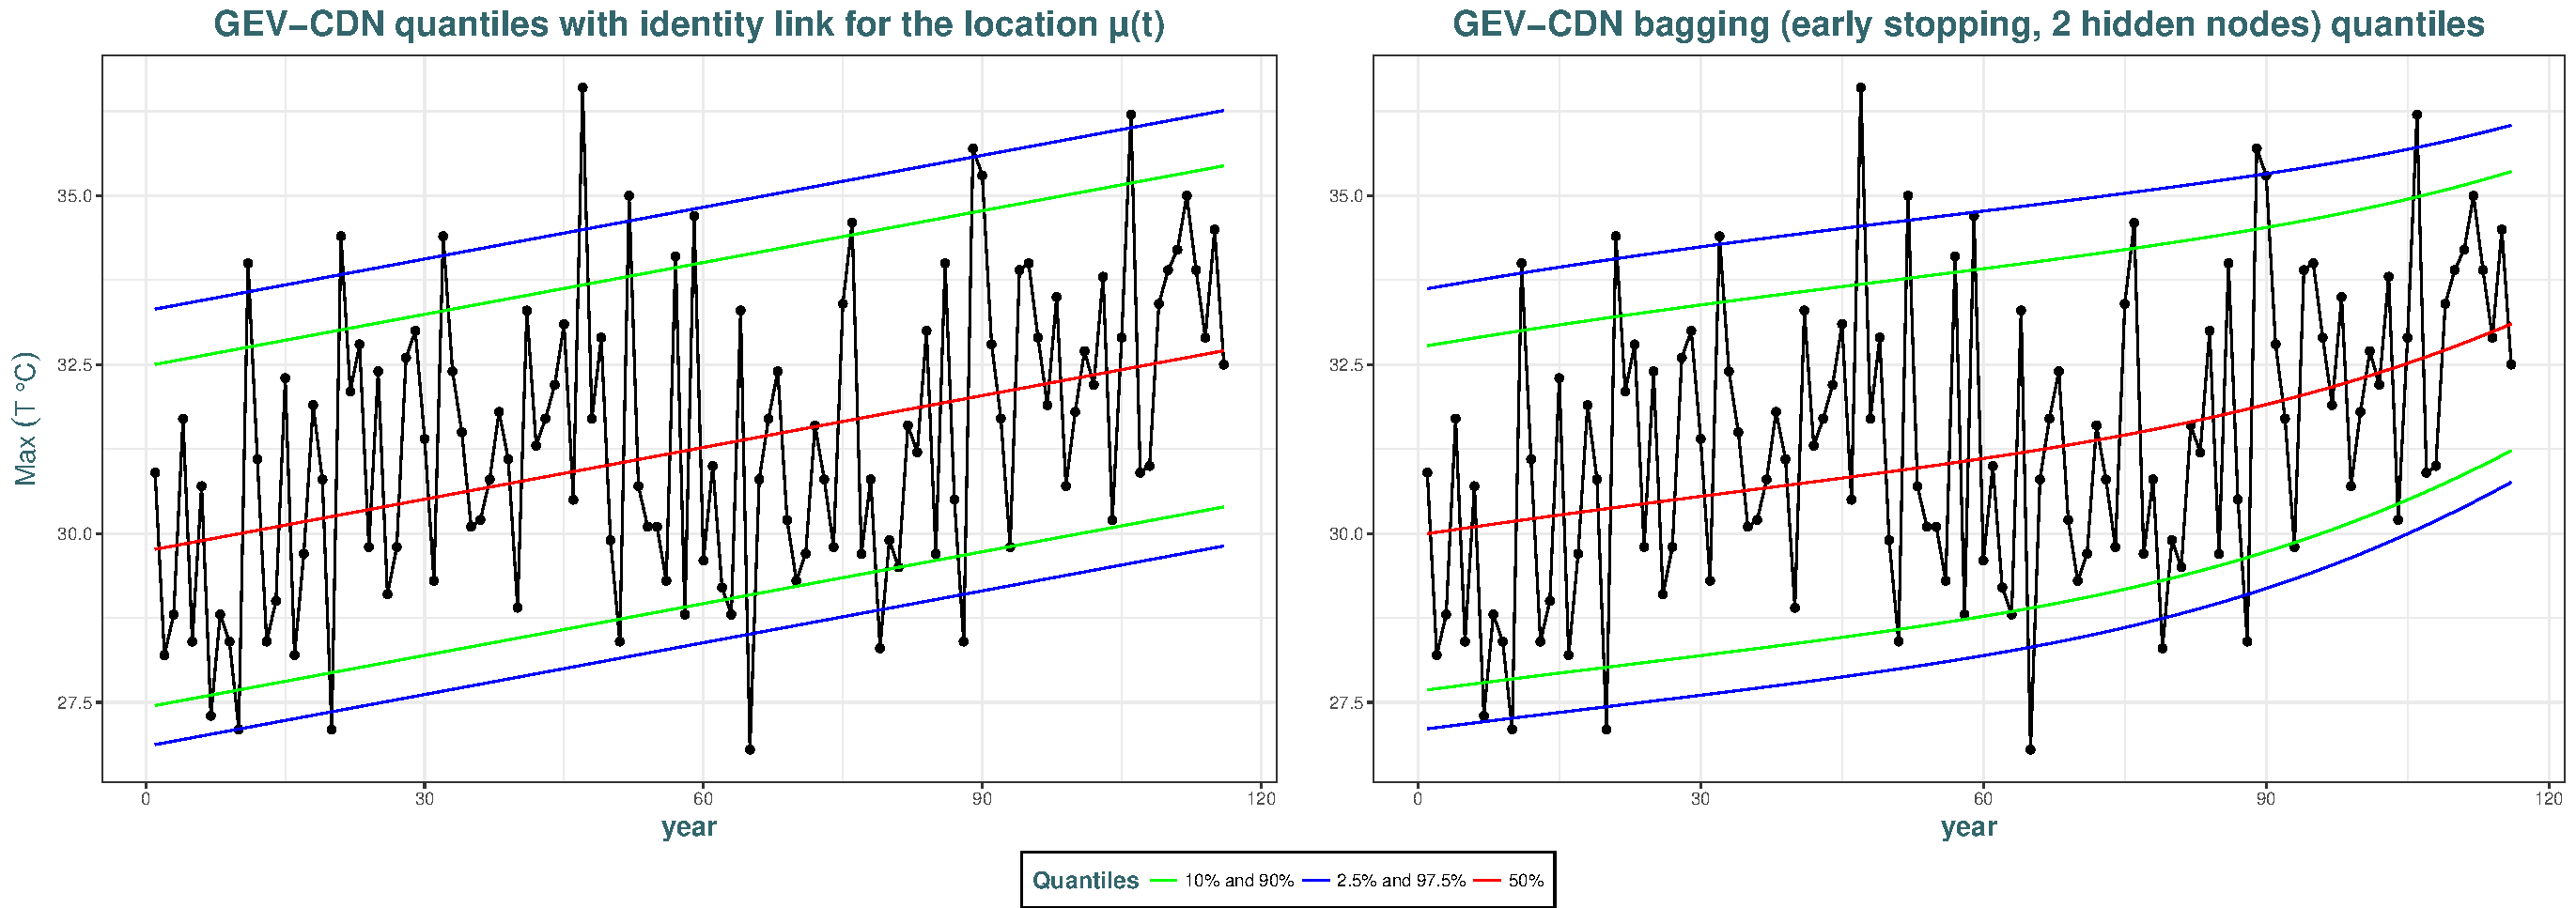
\includegraphics[width=1\linewidth]{gev_compv0.pdf}\caption{(Left) observations with quantiles from Model \ref{mod222} estimated in Table \ref{tab:estliknsta}. (Right) observations with same quantiles coming from the nonstationary and nonlinear bootstrap aggregated model with $M=1000$ resamples.
 	Note that in a stationary context, the $50\%$, $90\%$ and $95\%$ quantiles represent return levels with return periods of $2$, $10$ and $20$ years respectively.}\label{fig:bag}
 \end{figure}
 
In Figure \ref{fig:bag} we can clearly see the introduced nonlinear relationships in the two parameters $\mu(t)$ and $\sigma(t)$ with time from the two hidden layers. Compared with the left plot where the nonstationary link is linear and in $\mu(t)$ only, it seems that the ensemble model leads to an accelerate increasing rate at the end of the series, especially for low quantiles. This seems appropriate since the warming seems to accelerate for this period, and it fits with the findings of   \hyperref[sec:splines]{Section \textbf{\ref{sec:splines}}}. More formal comparisons could be made, for example \citet{cannon_flexible_2010} compared predicted quantiles  of the model with the empirical quantiles and computed the root mean squared error.


Note that the displayed values of the quantiles that are different for each year and represent return levels, can also be seen as confidence intervals, similar to credible intervals seen in the Bayesian paradigm in \hyperref[bayes_cred_int]{Section \textbf{\ref{bayes_cred_int}}}.
 
  In order to reduce the risk of overfitting, another technique that is commonly used is  \emph{weight penalty regularization}. In the \texttt{GEVcdn} framework, it works by controlling the variance $\sigma^2_w$ of a gaussian prior on the weights. %(in gev.fit or also gev.bag)
 Ideally, this value should be controlled by cross validation. It means that we have to find the value of $\sigma_w$ that provides the best fit relying on some criterion but this method rules out the use of the selection criterion such as BIC or $\text{AIC}_{\text{c}}$ since the effective number of model parameters will no longer be equal to the number of weights in the GEV CDN model. We chose $\sigma_w=2$ to limit the risk of overfitting. At the limit when $\sigma_w$ goes to zero, we checked that results are the same as for nonstationary GEV-CDN in location with no hidden layers, i.e. left plot of Figure \ref{fig:bag}.
 
%\textbf{ Finish the shiny application !!!! }
 
\subsection{Inference : Confidence intervals by Bootstrap }\label{sec:boot}
 
 
 
 \begin{figure}[!htb]
   	\centering	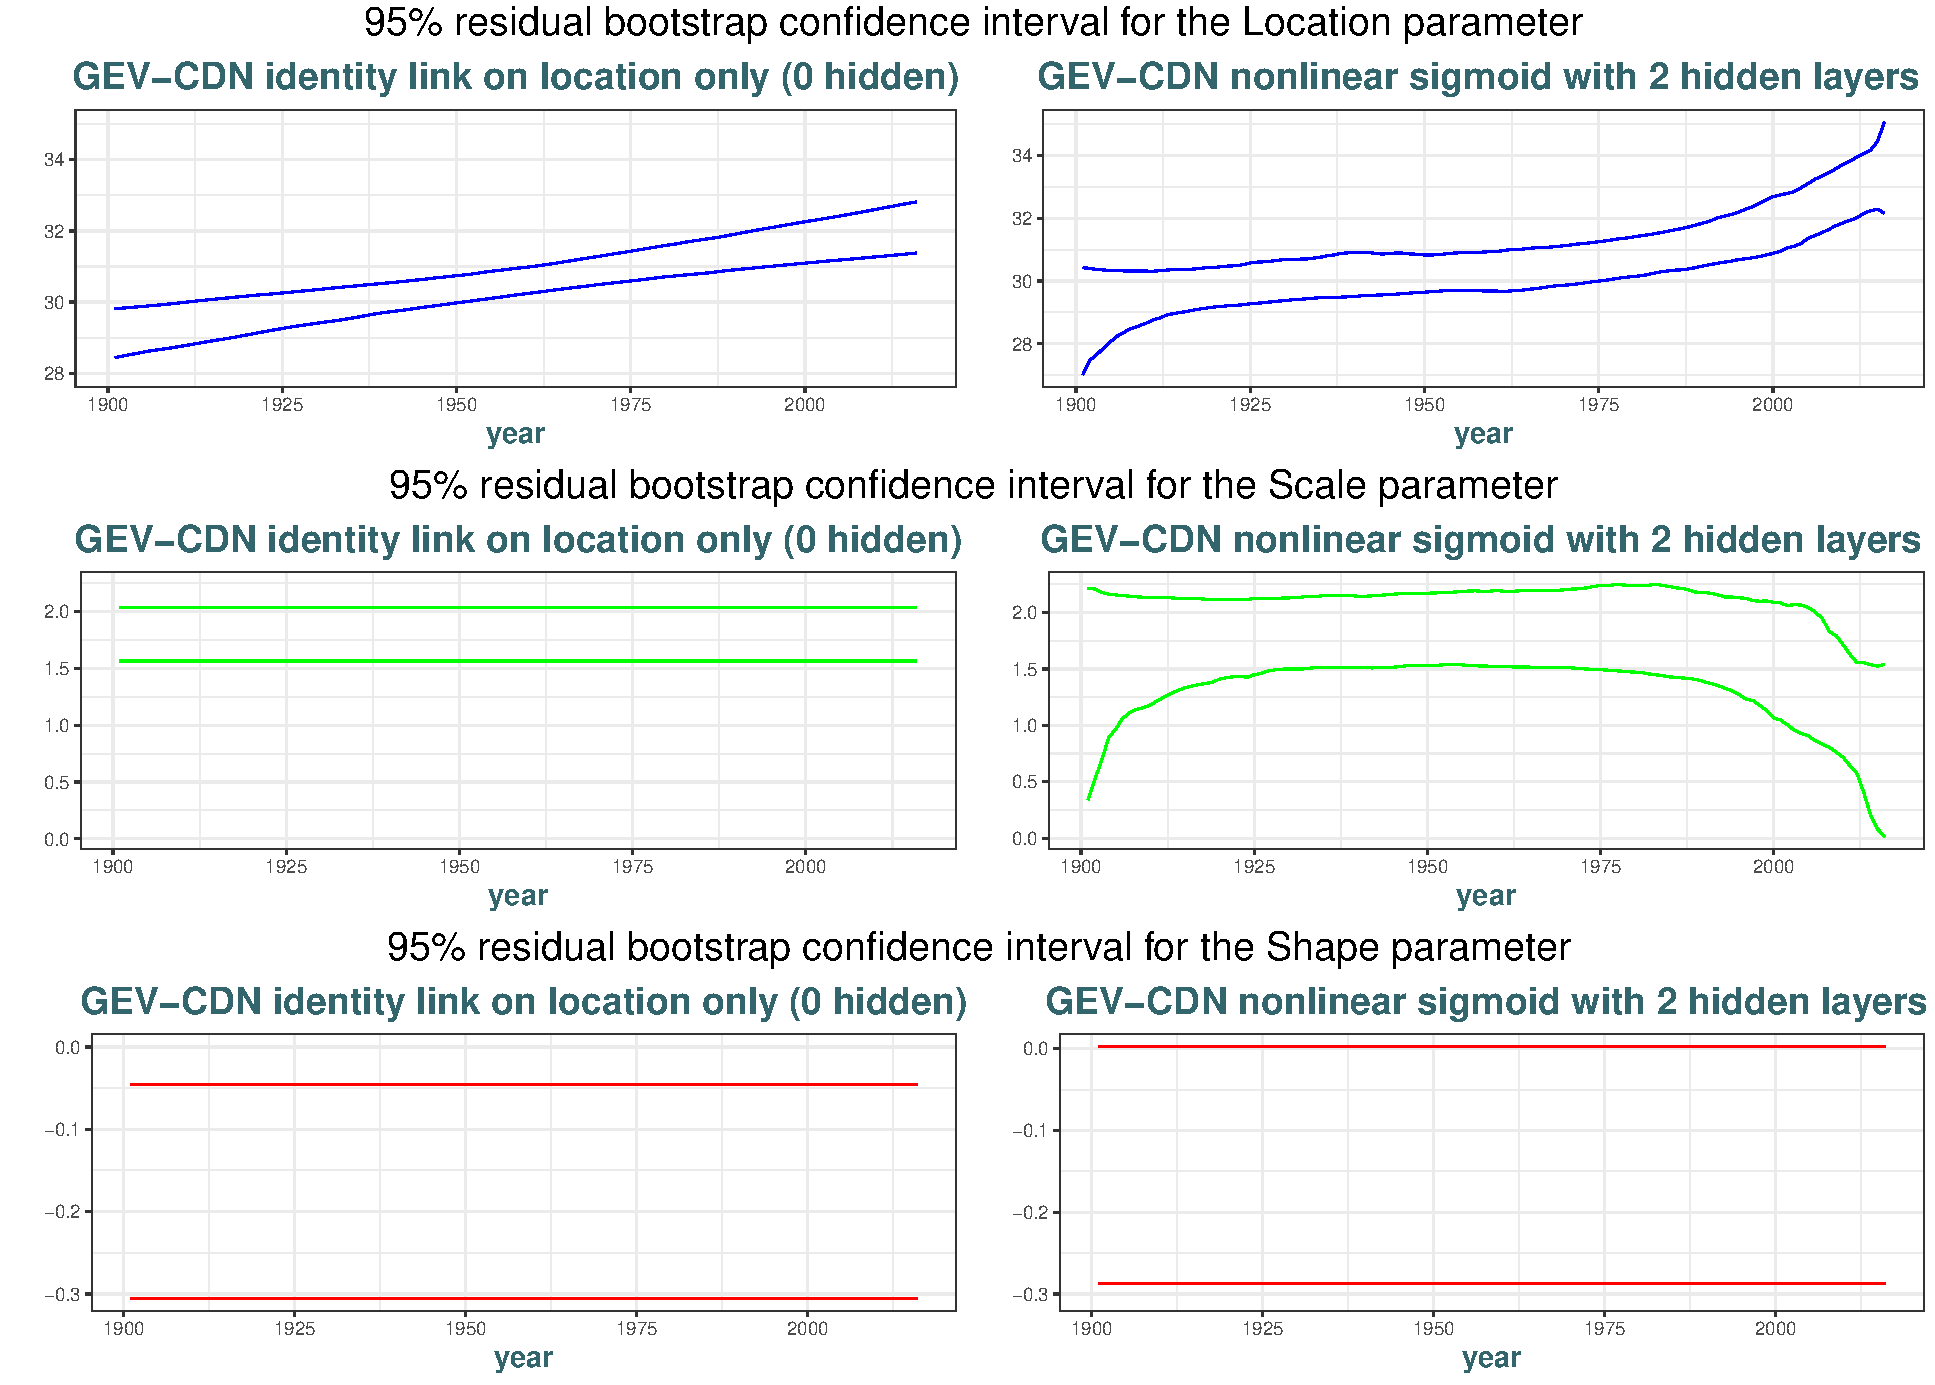
\includegraphics[width=1.01\linewidth]{g_boot_res.pdf}\caption{\textbf{Residual} bootstrap $95\%$ intervals computed with the GEV-CDN model allow a linear nonstationary location parameter only (left), and for the nonlinear nonstationary model in location and scale parameters only with 2 hidden layers (right). }\label{fig:boot_res}
 \end{figure}
   
 Bootstrap is an effective technique to compute accurate quantile-based confidence intervals when we cannot rely on approximations.
Similarly as for bagging, we did the computations in parallel. 
We took $B= 1000$ resamples in $74$ seconds for the residual bootstrap.
We used the residual bootstrap as presented in \hyperref[sec:nnboot]{Section \textbf{\ref{sec:nnboot}}} 
since it is the method recommended by \citet{kharin_estimating_2005}. The results are shown in Figure \ref{fig:boot_res} for all three GEV parameters, where left plots come from the $2.5\%$ and $97.5\%$ quantiles of Model \ref{mod222} (Table \ref{tab:estnn}) and right plots are for the nonlinear GEV-CDN model considered in the previous section (Table \ref{tab:estnnbag}) but with no bagging since it is not relevant to combine two bootstrap methods. We compared results with the parametric bootstrap from Figure \ref{fig:boot_par} left in \hyperref[app:fig]{Appendix \textbf{\ref{app:fig}}} but we note no significant differences. Graphs of the differences between the two methods did not yield additional concerns and are thus left at the end of \texttt{/Scripts-R/2NeuralsNets.R}. We think a coverage analysis is thus not relevant.
 These models have been chosen from previous sections. 
We did not extrapolate beyond the range of data.
 
 We clearly notice the flexibility introduced in the location and scale parameters intervals with the incorporated hidden layers. Stationary parameters have constant confidence lines as expected.
 Regarding the shape parameter $\xi$, we see that the value of $0$ is near to be outside the EV-Weibull type for the complex model. Moreover, we notice that this interval is wider for the complex model, but also regarding the location and scale parameters. To a certain extent, this loss of accuracy is due to overfitting, emphasized by the fact that we did not use bagging to estimate the model. We also note the decreasing behavior of the intervals for the scale parameters. This explains, to a certain extent, the decreasing quantiles intervals widths at the end of the series of right plot of Figure \ref{fig:bag}.

%Remark that we did not use bagging here  and that explains why the results are not as smooth as in the previous section 
  
 
 
\section{Comments and Comparisons with POT}


During this whole chapter, we considered time as the sole covariate. We recall that other covariates could have been included to improve the nonstationary analysis. To name a few : \emph{Southern Oscillation Index} (a proxy for El Niño), the $\text{CO}_2$ concentration, etc. Most of these are time-dependent.

There are many ways to analyze and we considered some of them. Sometimes our choices were subjective and thus debatable and this is the reason why we wanted to provide the user automated methods to easily redo analysis and visualize the effects of changing some of the (hyper)parameters.

The other approach we have seen in \hyperref[sec::2]{Chapter \textbf{\ref{sec::2}}} is the POT, and results were consistent with GEV for the EVI $\xi$ in the stationary and nonstationary analysis. For the nonstationary analysis, we considered e.g. varying thresholds and seasonal models.
A few results of nonstationary analysis in a POT approach are presented in Section 4.1 of the \texttt{Summary1\_intro.html} file in the \textbf{/vignettes} folder of the \href{https://github.com/proto4426/PissoortThesis/}{repository}. Threshold selection were an issue.


